%!TEX root = ../../secondYearReport.tex
\paragraph{Work package 2 progress}

\subparagraph{Definition and design of experimental protocols (T2.1)}

The aim of the work in this task was to provide a solid multidisciplinary base for future research work within CoDyCo. We made a thorough review and summary of the recent relevant literature on human postural control and whole body motion in contact with environment (Delivery 2.1). The review examines postural control strategies without and with additional support contacts, types of perturbations that are commonly used to study neuromuscular functions involved in postural control and reviews the methods for stability evaluation of bipedal systems. The review is concluded with examination of stability metrics that can be applied for non-planar contacts. We plan to extend the review with methods of determination of inertial parameters of human/robot body and submit it for publication in a robotic journal by the end of 2014.

At JSI, we created an experimental setup to study human postural control and whole body motion in contact with environment. We implemented two state-of-the-art methods for perturbation of balance as shown on Figure \ref{fig:exp_protocol_W2} that will allow us to gain understanding how human brain deals with environment in the sense of supportive contacts. Using the same setup we can also validate all biomechanical findings on robotic systems by simply substituting the human subject with a robot. Besides, work has been undertaken to setup experiments also at UB. New equipment (the Moog Hapticmaster robot) was acquired and configured at both JSI and UB. Hapticmaster robot will be used in experiments with compliant and unpredictable contacts.


\subparagraph{Design of models for human whole body motion in contact (T2.2)}

Work has begun on understanding how to derive simplified models of whole-body balance that will encapsulate the task relevant parameters of posture control with multiple contacts. By emulating situations when balance of an individual is challenged, we examined functional role of supportive hand contact at different locations where balance of an individual was perturbed by translational perturbations of the support surface. The experimental methods rested upon our work in Task 2.1 and are depicted on the left side of Figure \ref{fig:exp_paper_W2}.


We found that an additional supportive hand contact significantly reduced the maximal displacement of the subject's centre of pressure (CoP) regardless of the position of the handle and the type of the perturbation. On the other hand, the position of the handle had no effects on the maximal CoP displacement (top right diagram on Figure \ref{fig:exp_paper_W2}) which is against the previous belief that the quality of postural control depend on the location of the hand contact \cite{Sarraf2014} and supports the idea that maintaining postural stability is the task of the highest priority and that the central nervous system does whatever necessary to keep the body balanced \cite{Winter1995}. Specifically, subjects always generated the required hand force, no matter where the location of the handle was, to keep the body balanced to the same extent. To get a better understanding of the functional role of supportive hand contacts, we examined the handle forces exerted by the subjects during the perturbation. In 
contrast with the effects on CoP, we found significant effects of perturbation direction, perturbation intensity and handle position on the maximal force in the handle (bottom right diagram on Figure \ref{fig:exp_paper_W2}). A manuscript with the results of the work in T2.2 was submitted for publication in Gait \& Posture journal in December 2013 and is under review \cite{Babic2014}.

To properly model all these findings we developed a reduced dimensional (6-link, planar) model of a humanoid to be used as an inverse dynamics model for computing joint torques from human experimental data. The detailed analyses based on this model are under way at JSI and UB.

A major challenge of this task is understanding how to determine and measure stability when a human or humanoid robot is in a multi contact situation. The state-of-the-art in postural stability uses traditional metrics such as centre of pressure or zero moment point. However these planar metrics do not apply when there are multiple non-planar contacts. In addition to reviewing the current literature (Task 2.1), we have begun development of new methods for measuring stability margins when a human or humanoid robot has multiple non-planar contacts.

\subparagraph{Human contact choice and learning through physical interaction (T2.4)}

In order to understand how humans make contact choice decisions (e.g. whether or not to initiate a hand contact, and where to place the hand), we need an estimation of joint torques as well as a metric of stability in various multi-contact situations. Thus the work we have begun in Task 2.2 in terms of both simplified models of postural control and metrics of stability, also apply for Task 2.4.

To understand the factors involved in human choice of contact utilization, we performed a series of experiments where the subjects were standing still with arms hanging freely at the sides. The parallel platform induced a randomly timed series of perturbations of different accelerations, velocities and displacements. The aim of the experiments was to investigate what profile of support perturbation forces the human to make a supportive hand contact with environment and how human chooses the location of the hand contact with regard to the direction of the perturbation. Interestingly, we found that the subjects reacted to every perturbation no matter how small or slow the perturbation was or what was the initial acceleration of the perturbation. The reactions were manifested as muscle twitches of shoulder or as unspecific arm motions that were unrelated to the proximity of possible support objects. The reactions occurred also at the smallest perturbations when no actual correction of balance was needed. Our 
experiments showed that these reactions are essentially protective reactions rather than reactions that have counterbalancing effects \cite{McIlroy1995, Corbeil2013}.

These reactions mask the real factors involved in human choice of contact utilization. We therefore altered the perturbation methods for our further experiments and designed continuous random perturbations in a frequency band that corresponds with typical human motion during postural control \cite{Nawayseh2006}. By doing so we excluded the effect of surprise that evoked the reflex reactions of humans. This will hopefully allow us to uncover the factors involved in human choice of contact utilization.

%T4.2 TUD 3PM
%Summary: 
%In collaboration with JSI, TUD studied whether supporting contacts
%in human arm reaching tasks are planned or an effect of a reactive controller. 
%Probabilistic inference in learned models of kinematics provide evidence for planned contacts in human reaching. 

%description of work:
\begin{figure}
\centering
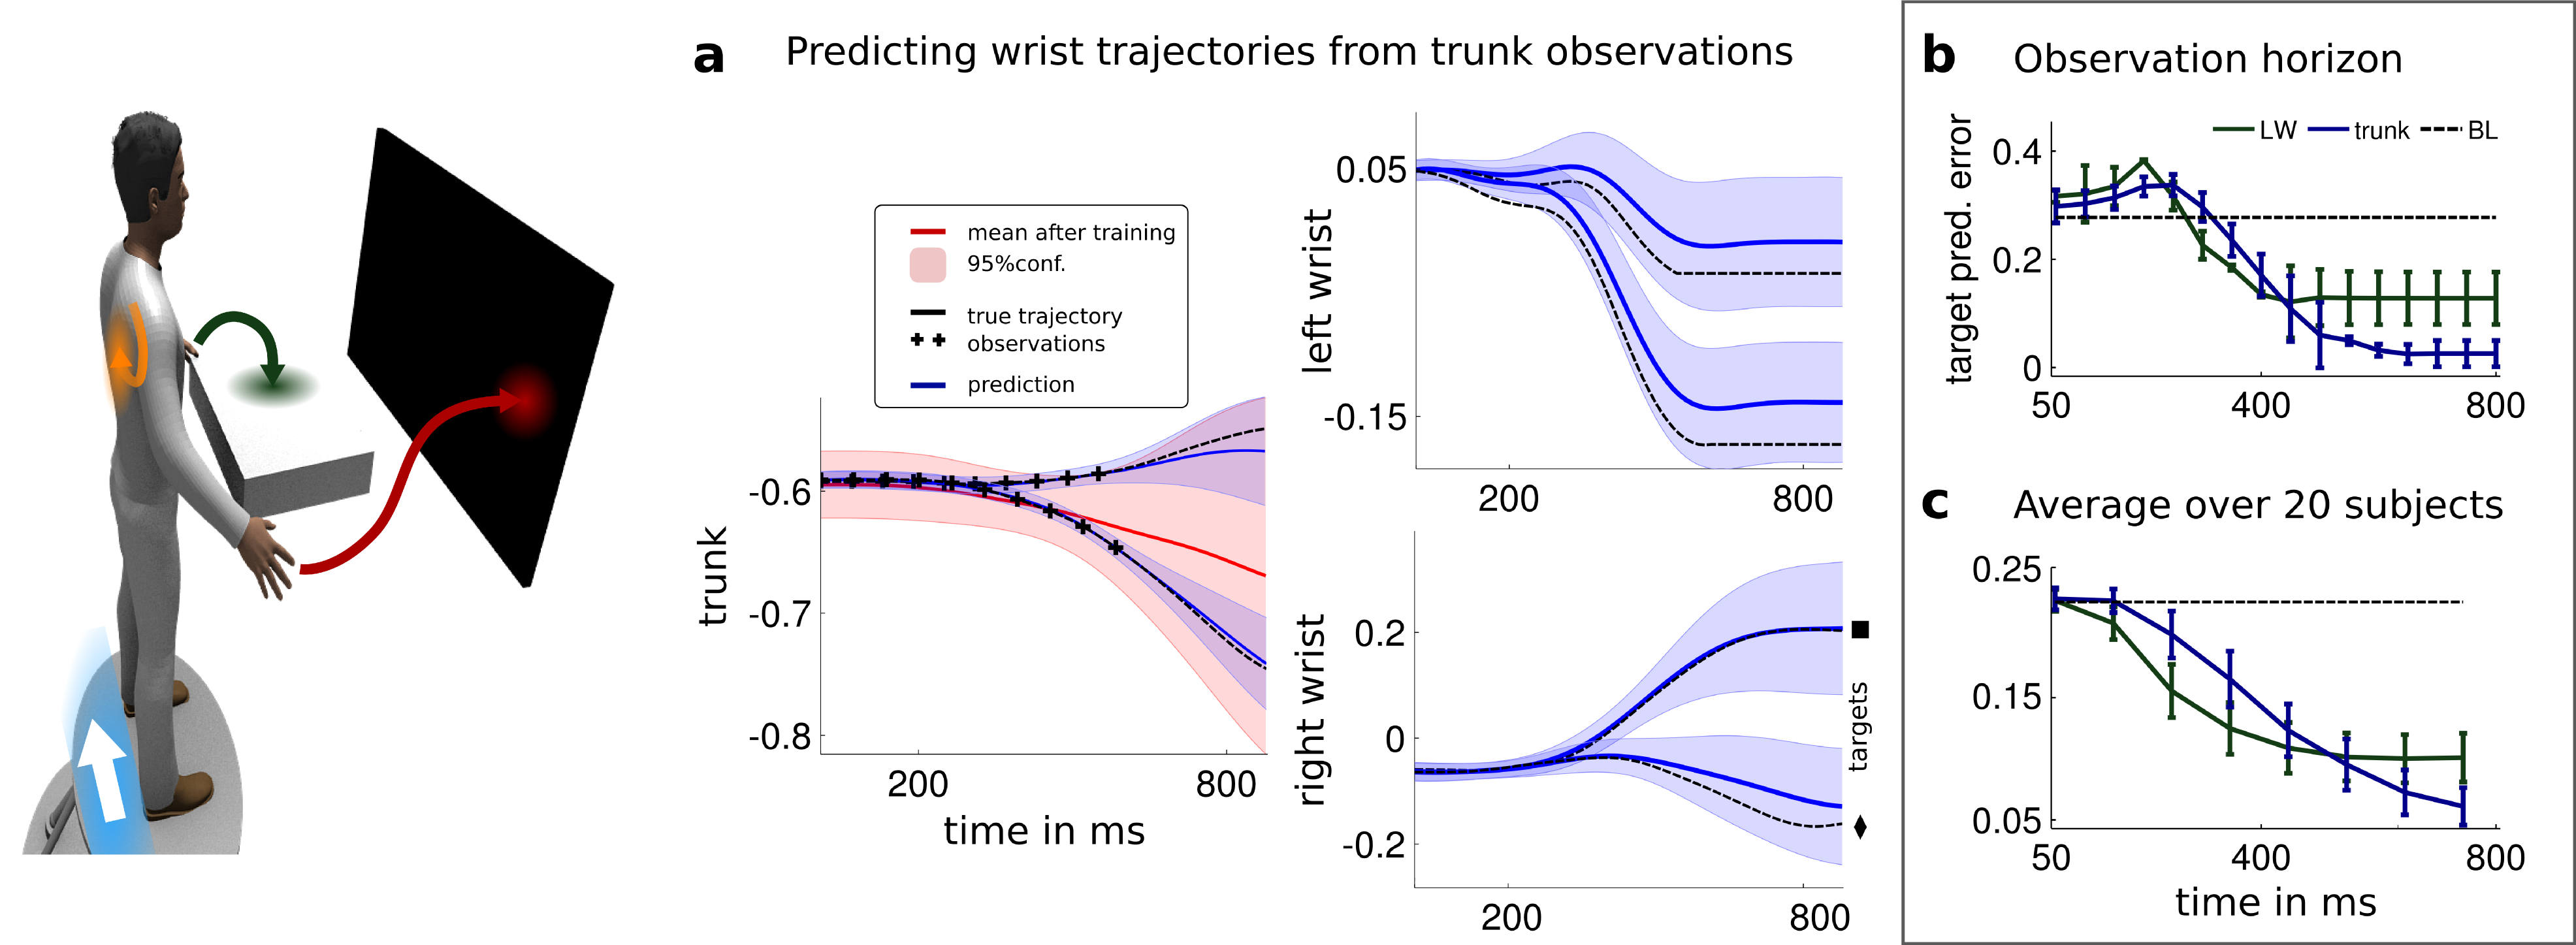
\includegraphics[width=0.8\textwidth]{./sections/WP2/pics_TUD/SummaryFig_Y2Report}
%\label{fig:subfig2}
 \caption{Trunk trajectories predict wrist trajectories.  
 (a) 600ms of trunk trajectories are observed. These observations can predict the wrist trajectories. Shown are predictions for the two exterior targets on the screen. 
 For training 10 trials for each target are used starting from trial 240 backwards in time (before the catch trials). For testing the first perturbed trial after trial number 240 were used. 
 (b) The effect of the observation horizon on the target prediction error is shown for a representative subject. The mean of the training data denotes the base line (BL). (c) Average statistics (mean and 95 percent confidence bound) over 20 subjects.
}
\label{fig:HumanProMPsPrediction}
\end{figure}
In collaboration with JSI, TUD studied whether supporting contacts
in human arm reaching tasks are planned or an effect of a reactive controller. 
Investigations on human motor learning has focused on adaptation experiments with fixed contact points leaving 
research on the computational role of contacts as a free control variable unexplored. 
In perturbed target reaching experiments sketched in Figure \ref{fig:HumanProMPsPrediction}, we studied weather supporting contacts are planned or reactive. 
Subjects had to reach for distant targets on a screen with their right hand. 
For reaching the target additional support through contacts with a table using the left hand was inevitably. 
If the contacts are planned then the left hand's motion can predict the right hand reaching. 
We studied how probabilistic inference in learned models can be used to answer this question. 
Evidence for planned contacts could be provided through learning probabilistic models of trajectory distributions and using the models to generate predictions, Figure \ref{fig:HumanProMPsPrediction} (a). 
We found that the target on the screen could be predicted from both, the left hand (mse: $10.4$cm $\pm$ $2$cm over $20$ subjects) and the trunk movement (mse: $6.7$cm $\pm$ $1.4$cm over $20$ subjects), which 
is illustrated in Figure \ref{fig:HumanProMPsPrediction} (b-c). 
The learned probabilistic model could also be used to analyse the rate of adaptation of the left hand and the trunk kinematics, 
where the trunk trajectories converged faster than the left hand motion. 
This is intuitively explained by the strong need for corrective trunk movements in balancing. 
A report on the findings is currently in progress of writting.

